
\section{The Approach}

\vfill


\begin{figure}[H]
  \centering

  % === First row ===
  \begin{subfigure}[t]{0.45\textwidth}
  \centering
  \begin{tikzpicture}
    \comicpanel{0}{0}
      {Founder}
      {Aquirer}
      {\small How would you describe your involvement — strategic or operational?}
      {(-0.6,-0.6)}
  \end{tikzpicture}
  \caption*{The probe begins.}
  \end{subfigure}
  \hfill
  \begin{subfigure}[t]{0.45\textwidth}
  \centering
  \begin{tikzpicture}
    \comicpanel{0}{0}
      {Founder}
      {Aquirer}
      {\small Our clients don’t hire us to execute. They hire us to unlock.}
      {(0.6,-0.6)}
  \end{tikzpicture}
  \caption*{The dodge.}
  \end{subfigure}

  \vspace{1em}

  % === Second row ===
  \begin{subfigure}[t]{0.45\textwidth}
  \centering
  \begin{tikzpicture}
    \comicpanel{0}{0}
      {Founder}
      {Aquirer}
      {\small What happens if we miss significant milestone?}
      {(-0.6,-0.6)}
  \end{tikzpicture}
  \caption*{The second probe.}
  \end{subfigure}
  \hfill
  \begin{subfigure}[t]{0.45\textwidth}
  \centering
  \begin{tikzpicture}
    \comicpanel{0}{0}
      {Founder}
      {Aquirer}
      {\small It wouldn't be a problem for you... because your decisions wouldn't matter anymore.}
      {(0.6,-0.6)}
  \end{tikzpicture}
  \caption*{The founder’s suspicion grows.}
  \end{subfigure}

  \caption*{\textbf{Not every offer is a gift. Some are blueprints for your own assimilation.}}
\end{figure}


\subsection{The Kind of Curiosity That Makes Money}

Michael Hart was in the audience.

Technically, he wasn’t supposed to be at the conference.

But a client meeting fell through. Instead of flying out early, he decided to walk the expo floor, 
kill time, and stay curious. 

He had the kind of curiosity that made money.

The place was all beige carpet, compostable coffee cups, and rows of booths hawking ``responsible AI''
and ``next-gen compliance intelligence.'' Hart stood out. He did not stand out because of the Tom Ford suit 
or the way he bypassed the espresso bar without slowing. 
He stood out because while everyone else was networking, he was listening.

He was really listening.

The speaker --- some founder, younger than he looked --- was pacing lightly. 

There were no theatrics. 

There was no cheap enthusiasm. 

There was just stillness and space. 

He wasn’t selling. 

He was building tension.

``Think of your last quarterly filing? I bet ninety percent of it was written by an LLM.''

There was no slide callout. 
He just showed statistics.

``You can tell which firms use which models,'' 
the man said. 
``And you can tell when the humans stopped writing.''

Now Hart was genuinely impressed.

Because this wasn’t just technical posturing. 
It was tactical.

``Your filings sound the same,'' 
the speaker continued, 
``because your models were trained on the same internet.'' 

A pause.

``Your reports collapse nuance because your prompts were rushed. 
And your junior analysts don’t push back because the model always says it `sounds confident'.''

He paused.

``And regulators are catching on.
They’re not just looking for fraud.
They’re looking for detachment.''

That word --- detachment --- lingered.

And then the founder said something Hart hadn’t expected to hear at a compliance conference.

``Heidegger called it the hermeneutic circle,'' the man said.

\begin{figure}[H]
  \centering
  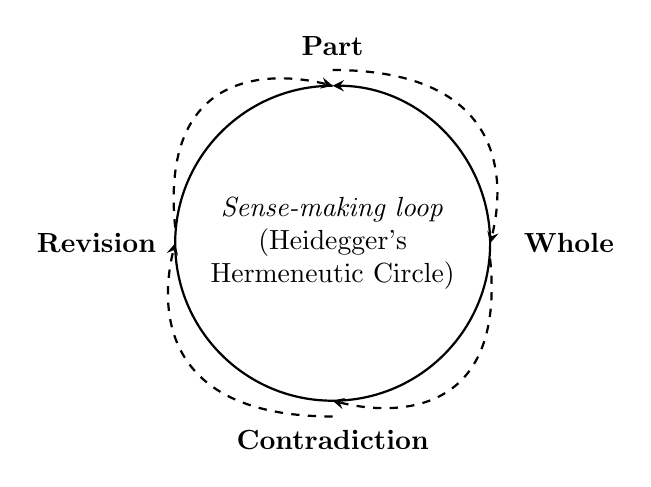
\begin{tikzpicture}[>=stealth, thick, node distance=2cm, every node/.style={align=center}]

    % Circle path
    \draw[->, thick] (0,2) arc[start angle=90, end angle=450, radius=2cm];

    % Labels on the circle
    \node at (0,2.5) {\textbf{Part}};
    \node at (3,0) {\textbf{Whole}};
    \node at (0,-2.5) {\textbf{Contradiction}};
    \node at (-3,0) {\textbf{Revision}};

    % Circular arrows to show motion
    \draw[->, dashed] (0,2.2) .. controls (2.2,2.2) and (2.2,0.8) .. (2,0);
    \draw[->, dashed] (2,-0.2) .. controls (2.2,-2.2) and (0.8,-2.2) .. (0,-2);
    \draw[->, dashed] (0,-2.2) .. controls (-2.2,-2.2) and (-2.2,-0.8) .. (-2,0);
    \draw[->, dashed] (-2,0.2) .. controls (-2.2,2.2) and (-0.8,2.2) .. (0,2);

    % Center text
    \node at (0,0) {\textit{Sense-making loop}\\(Heidegger’s\\Hermeneutic Circle)};

  \end{tikzpicture}
  \caption{The Hermeneutic Circle: Understanding emerges through iterative interpretation between part and whole.}
\end{figure}


A few faces shifted in confusion.

``It’s the idea that our understanding of any part of something 
--- a number, a signal, or a trade --- 
depends on our understanding of the whole. 
And our understanding of the whole depends on how we interpret the parts.''

He gestured toward nothing in particular. It was more a gesture of thought than performance.

``That’s how humans make sense of the world.
We don’t discover meaning. We assemble it: contextually, relationally, and iteratively.''




He let the idea hang a moment longer.

Then he offered an example.

\begin{quote}
``Imagine you’re reading a quarterly earnings report,'' he said.  
``And everything looks fine—growth’s steady, margins are good, guidance is confident.''
\end{quote}

A few heads in the audience nodded.

\begin{quote}
``But then one line catches your eye:  
‘Accounts receivable increased 41\% year-over-year.’''
\end{quote}

He paused, just long enough.

\begin{quote}
``That doesn’t fit the story. Not if the rest of the picture shows efficiency.  
So now, the whole doesn’t make sense.  
And you're forced to circle back—ask why.  
Did they delay collections? Extend terms? Book revenue early?''
\end{quote}

Another pause.

\begin{quote}
``The contradiction forces a reinterpretation—of the part \textit{and} the whole.''
\end{quote}

Now Hart was still. Fully still.

\begin{quote}
``Maybe you revise your understanding of the quarter.  
Maybe you go back to the transcript and listen for what wasn’t said.  
Maybe you call someone in the supply chain.’’
\end{quote}

He shrugged, as if this were obvious.

\begin{quote}
``That’s how real analysts work.  
They don’t just parse outputs. They \textit{interact} with inconsistencies.  
They engage in a loop: revise the map or revise the terrain.  
And eventually, the picture clarifies—because it has to.''
\end{quote}

He took a slow breath.

\begin{quote}
``The hermeneutic circle isn’t just philosophy.  
It’s how sense-making works—in markets, in systems, in people.''
\end{quote}

He let the silence settle.

\begin{quote}
``That’s what our models don’t do yet.  
Not really.  
They don’t get \textit{uneasy} when the parts don’t match the whole.''
\end{quote}

Now the room was quiet.

Even the people near the espresso bar had stopped pretending to multitask.

And Hart?

Hart wasn’t evaluating the product anymore.

He was evaluating the founder.






It was a rare thing to hear someone in AI talk about meaning as something earned, not extracted.

``Heidegger warned that modern systems 
--- especially powerful ones --- 
flatten this process.
They frame the world as inventory.
They optimize, index, and abstract until the forest becomes a yield chart.
Until understanding becomes a query.''

Hart didn’t need it spelled out.

If meaning was assembled —-- not discovered --- then every automated compliance system built on 
detached extraction was, by design, brittle. AI that parsed policies, flagged exceptions, or 
generated audit narratives without context wasn’t just fallible. It was philosophically blind. 
It couldn’t understand the why behind a transaction, only the what. 
And in compliance, the why was everything. 
If the system couldn’t interpret intent... 
and couldn’t weigh contradictions... 
and couldn’t pause to reconcile the part with the whole then it couldn’t regulate. 
It could only recite. 
Which meant that most AI compliance platforms weren’t actually protecting firms from risk. 
They were just accelerating the process of misunderstanding it.

\subsubsection{Horizons Don’t Collapse — They Meet}

The founder let the silence do its work, then moved forward carefully — like someone who knew the room could follow him just a little further.

``Heidegger laid the groundwork,'' he said.  
``But it was Gadamer who extended it.''

A few audience members shifted. A name fewer had heard.

``He argued that interpretation isn’t just circular. It’s historical. Situated. Dialogical.''

He paced again, but slower now — not to move, but to let the idea move through the room.

``He called it a fusion of horizons.''

\medskip

\begin{figure}[H]
  \centering
  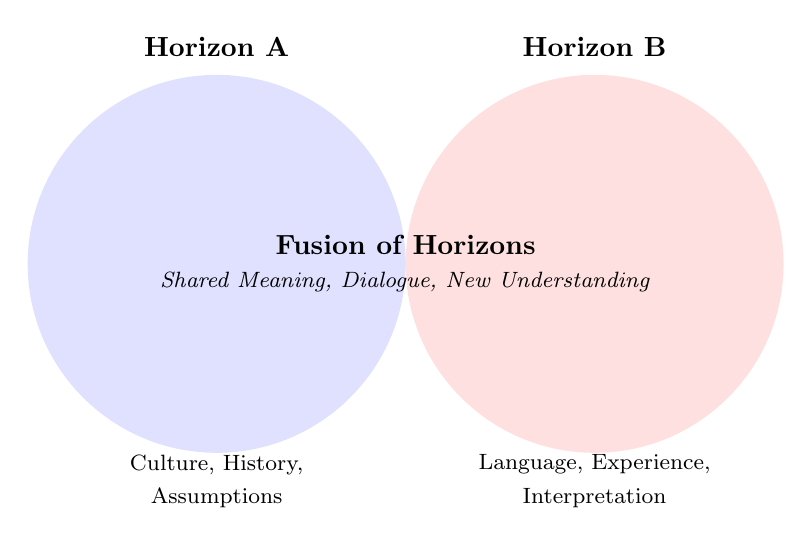
\begin{tikzpicture}[scale=1.2, thick]
    % Horizon A
    \begin{scope}
      \fill[blue!20, opacity=0.6] (-2,0) circle (2cm);
    \end{scope}
    \node at (-2,2.3) {\textbf{Horizon A}};
    \node[align=center] at (-2,-2.3) {\footnotesize Culture, History,\\ \footnotesize Assumptions};

    % Horizon B
    \begin{scope}
      \fill[red!20, opacity=0.6] (2,0) circle (2cm);
    \end{scope}
    \node at (2,2.3) {\textbf{Horizon B}};
    \node[align=center] at (2,-2.3) {\footnotesize Language, Experience,\\ \footnotesize Interpretation};

    % Overlap manually using path instead of clip
    \begin{scope}
      \clip (-2,0) circle (2cm);
      \fill[orange!50, opacity=0.7] (2,0) circle (2cm);
    \end{scope}

    % Label for fusion area
    \node[align=center] at (0,0) {\textbf{Fusion of Horizons}\\\textit{\footnotesize Shared Meaning, Dialogue, New Understanding}};

  \end{tikzpicture}
  \caption{Gadamer’s Fusion of Horizons: Interpretation arises when perspectives overlap and co-construct meaning.}
\end{figure}


\medskip

He turned to the audience, less professorial now. More intimate.

``Each of us stands inside a horizon — a boundary of assumptions, knowledge, and perspective that shapes how we see the world. That horizon isn’t fixed. It’s formed by culture, memory, language, and context.''

He paused.

``When we encounter something unfamiliar — a foreign text, a contradictory number, a decision we don’t yet understand — our first instinct is to make it fit \textit{our} horizon.''

He let that land.

``But Gadamer says real understanding comes when we let the horizon of the other meet our own. Not to erase it. Not to dominate it. But to allow a fusion — a widening of context that makes new sense possible.''

Now he was fully in control of the room.

``That’s why interpretation isn’t about certainty. It’s about negotiation.  
Between present and past. Between part and whole. Between reader and signal.''

Then he brought it back.

``In compliance, that matters. Because regulations have a horizon. So do markets. So do people.  
And so does the AI you use to make sense of all three.''

He took a breath.

``If your model can’t hold two horizons in tension —  
if it can’t pause at the edge of what it knows and reach toward what it doesn’t —  
then it can’t interpret.  
It can only translate.''

And that was the difference.

Translation renders content.\\
Interpretation renders meaning.


And meaning — in a system built on intent, ambiguity, and context — was non-negotiable.

Michael Hart didn’t nod. He didn’t blink.

He had heard a lot of founders pitch certainty.  
But very few were fluent in the language of earned ambiguity.

Fewer still could speak it fluently while watching the room shift with them.

Hart was no longer curious.

He was invested.

\medskip


\begin{PhilosophicalSidebar}{Gadamer's Horizons — Understanding as a Dialogical Act}

  Hans-Georg Gadamer extended Heidegger’s hermeneutics by introducing the idea of the \textbf{fusion of horizons}.  
  A \textbf{horizon}, in Gadamer’s terms, is the scope of vision that includes everything we can understand — 
  a boundary shaped by our language, culture, history, and assumptions.
  
  \medskip
  
  Understanding doesn’t happen by erasing these horizons or imposing one over another.  
  It emerges through a dialogical process — where conflicting perspectives encounter each other, 
  adjust, and \textit{fuse} into something larger and more coherent.  
  
  \medskip
  
  \textbf{Interpretation}, then, is not decoding a fixed truth.  
  It’s engaging in an evolving conversation between what we know and what we’re learning.  
  It’s an act of openness — not just to information, but to transformation.
  
  \medskip
  
  \textbf{In the context of AI and compliance:}
  
  \begin{itemize}
    \item A regulation has a horizon — its legal context, intent, and socio-political roots.
    \item A firm has a horizon — its operational models, culture, and incentive structures.
    \item An AI system has a horizon — defined by its training data, architecture, and assumptions.
  \end{itemize}
  
  \medskip
  
  Most AI systems don’t engage these horizons.  
  They flatten them.  
  They treat regulations as text, not context.  
  They treat human decisions as signals, not negotiations.  
  And in doing so, they simulate compliance — without actually understanding it.
  
  \medskip
  
  Gadamer’s insight is that real understanding happens when horizons are allowed to meet —  
  not by force, but by interpretation.
  
  \textit{Without that, AI can execute rules, but it can’t reconcile meanings.  
  It can parse the surface, but not participate in the conversation beneath it.}
  
\end{PhilosophicalSidebar}

\medskip





The founder paused.

``And that’s what we’ve done with enterprise AI.
We’ve built models that respond without awareness.
That complete without comprehension.
That predict... without pausing.''

Then the pivot came, clean and sharp:

``That’s why we didn’t just train a model.
We raised one.''







The phrasing was deliberate, and it made Hart’s ears lift.

``You can’t just feed SEC filings into a transformer and expect a junior analyst. You get parrots.''

Hart knew this already. 
Everyone in the room did. 
However, no one had said it that cleanly. 
And no one had said what came next.

``We built NPC mentors. 
Simulated analyst chatrooms. 
We gave the model redlined narratives and synthetic feedback from fake supervisors. 
We didn’t just teach it tasks. 
We gave it a synthetic childhood.''

That was the moment Hart looked at the man’s face differently.

This wasn’t someone trying to disrupt enterprise software. 
This was someone reimagining cognitive development --- at scale --- inside machines.

The founder gestured toward a timeline projected behind him, though he barely looked at it himself.

``We modeled the first 18 months on the job. 
Not just output. 
But what it feels like to be wrong. 
To defend a bad idea. 
To hesitate mid-sentence.''

He paused, then added, almost offhandedly:

``The inspiration wasn’t enterprise AI. It was Jean Piaget.''

That caught even Hart by surprise.

``Piaget didn’t think children absorbed knowledge. 
He believed they constructed it... through contradiction... and through conflict... and through play.''

\medskip

\begin{PsychologicalSidebar}{\textbf{Cognitive Development and the Piagetian Arc}}

  Jean Piaget, a Swiss psychologist, revolutionized our understanding of how humans acquire knowledge. Rather than seeing children as miniature adults, Piaget proposed that they progress through distinct stages of cognitive development, each with its own logic, limitations, and forms of reasoning.

  \medskip
  
  \begin{itemize}
  \item \textbf{Sensorimotor Stage (0–2 yrs)} — Learning through direct experience. Cause and effect is discovered through physical interaction (e.g., kicking a mobile and watching it move).
  \item \textbf{Preoperational Stage (2–7 yrs)} — Language emerges, but thinking is still egocentric and symbolic. Children can mimic and imagine but struggle with logic and perspective-taking.
  \item \textbf{Concrete Operational Stage (7–11 yrs)} — Logical thinking begins, tied to tangible situations. Children can categorize, reverse operations (e.g., 4 + 2 = 6 so 6 – 2 = 4), and begin to grasp rules and structure.
  \item \textbf{Formal Operational Stage (12+ yrs)} — Abstract reasoning becomes possible. Hypotheticals, counterfactuals, and systematic planning emerge. Thought becomes metacognitive — one can think about thinking.
  \end{itemize}

  \medskip
  
  These stages aren’t just biological — they reflect an interaction with the world. Knowledge isn’t absorbed; it’s constructed through play, contradiction, and recalibration.

  \medskip
  
  \textbf{In synthetic systems, Piaget’s insights remain relevant.} If you want a machine to reason like a human, you can’t just feed it more data. You have to simulate these developmental arcs: imitation, failure, revision, and abstraction.

  \medskip
  
  In essence, true intelligence isn’t formed by stacking facts — it’s built by recovering from being wrong.
  
\end{PsychologicalSidebar}

\medskip

The room was quiet.

``And we did the same. 
We didn’t fine-tune on task data. 
We walked the model through Piaget’s cognitive stages.''

Hart recognized the names now, as the founder spoke them aloud:
\begin{itemize}
  \item Sensorimotor. 
  \item Preoperational. 
  \item Concrete operational. 
  \item Formal operational.
\end{itemize}

Each one grounded not in abstraction, but in training methodology.

``In the sensorimotor stage,'' 
he said, 
``we used reactive correction. 
If the model made a trade that failed in simulation, it got slapped.''

Then:

``Preoperational meant language mimicry. 
So we fed it analyst slack logs. 
The chatter. 
The gossip. 
The flawed logic that still kind of works. 
We didn’t care if it was perfect. 
We cared that it was human.''

Hart caught the implication: this founder wasn’t optimizing for clarity. 
He was optimizing for contextual fluency.

``Concrete operational? 
That was conflict. 
We built fake colleagues. 
Forced it to explain itself. 
We made it justify risk. 
Defend bad assumptions. 
Get called out. 
And recover.''

And then, finally:

``Formal operational — the highest stage. 
We gave it abstract models. 
Shadow portfolios. 
Failed strategies. 
We didn’t ask for predictions. 
We asked for counterfactuals. 
For what-ifs.''

The founder took a small step away from the podium now, letting the quiet settle.

``We weren’t training a typist,'' he said. ``We were cultivating judgment.''

And then he said the thing that Hart would quote later, word for word, to his lieutenants back at Centauri:

``Not just: `How do you complete this task'? But: `Why would a human pause right here'?''

He tapped the side of his head.

``That pause? That hesitation? That’s where the real learning happens.''

He let the moment breathe.

Then, more quietly now—less like a presenter, more like someone letting the room in on a hard truth:

“Because that hesitation? That flicker of doubt?”

He glanced toward the audience.

“That’s the difference between compliance as protocol… and compliance as comprehension.”

Now a few people leaned in.

David didn’t pace. He just stood there, anchored.

“A regulator doesn’t care that you followed the steps. Not really.
They want to know if you understood what the steps were for.
They want to know if someone — anyone — had the presence of mind to pause.”

His tone tightened. Not aggressive. Surgical.

“When the numbers spiked.
When the exposure changed.
When the model suggested a trade that was technically correct but morally wrong —
did anyone stop?”

He let the question land.

“Because compliance isn’t about detection.
It’s about discretion.”

A beat.

“And discretion isn’t found in the output.
It’s found in the hesitation before the output.”

He tapped his temple again.

“Regulators don’t want a log of what happened.
They want a trace of awareness.
A signal that the system knew why it was doing what it did—
or that a human was close enough to intervene when it didn’t.”

He looked directly at the front row now.

“If your system can’t model that moment—
the pause, the contradiction, the unease—
then you’re not automating compliance.

You’re anesthetizing it.”

Then, gently:

“This isn’t an automated decision tool.
It’s not meant to replace judgment.
It’s meant to amplify it.”

He stepped forward again, his voice steady:

“It’s a mentor, not a manager.
A second brain.
A partner that knows just enough to nudge when you forget to ask the obvious question.”

Another pause.

“That’s what regulators are actually looking for.
Not just evidence that you followed procedure—
but evidence that you noticed something when the procedure wasn’t enough.”

He exhaled slightly.

“And if your system can’t support that kind of noticing?
Then it’s not augmentation.
It’s abdication.”

\medskip

\begin{HistoricalSidebar}{\textbf{SVB, KPMG, and the Cost of Not Pausing}}

  In March 2023, Silicon Valley Bank collapsed in what became the second-largest bank failure in U.S. history. 
  It wasn’t alone. Signature Bank fell days later. First Republic followed. Panic rippled. 
  Confidence cracked. For a few weeks, the phrase ``contagion risk'' re-entered the mainstream 
  (Huang \& Nasiripour, 2023).

  \medskip
  
  But one of the more quietly unsettling aspects of the SVB collapse wasn’t the speed.
  It was the signatures.

  \medskip
  
  
  Specifically: KPMG.

  \medskip
  
  
  The global accounting firm had recently issued clean audit opinions for both SVB and Signature Bank. 
  No major red flags. No raised alarms. No hesitation (Eavis, 2023).

  \medskip
  
  
  At the time, that stamp of approval was supposed to inspire trust.
  To many, it did the opposite.

  \medskip
  
  
  Because the deeper critique wasn’t about negligence. It was about obedience.
  KPMG did everything it was supposed to do.

  \medskip
  
  
  And that, some argued, was exactly the problem.

  \medskip
  
  
  While other auditors flagged liquidity mismatches and duration risks using broader judgment, 
  KPMG stuck to formal procedure. They tested controls. Verified disclosures. Cross-checked spreadsheets. 
  They followed the rules.

  \medskip
  
  
  They didn’t flinch.

  \medskip
  
  
  They didn’t pause.

  \medskip
  
  
  They didn’t ask whether the underlying risk had shifted meaning — whether it had outgrown the template 
  it was being measured against.

  \medskip
  
  
  In other words: they didn’t interpret.

  \medskip
  
  
  To some, this wasn’t a failure of audit.
  It was a failure of awareness (Son, 2023).

  \medskip
  
  
  The lesson?

  \medskip
  
  
  \textit{Doing what you’re supposed to do} is not the same as knowing when what you’re doing no 
  longer makes sense.

  \medskip
  
  
  That’s the difference between protocol and prudence.
  Between detection and discretion.
  Between automation... and judgment.

  \medskip
  
  
  And in the end, it wasn’t the lack of process that brought those banks down.

  \medskip
  
  
  It was the lack of interruption.
  
\end{HistoricalSidebar}

\medskip







Hart let out the smallest breath.

This wasn’t a founder looking for funding.

This was someone who had already solved a problem most firms hadn’t even realized they had.

That was the moment Hart decided.

This wasn’t another AI play. 
This wasn’t someone chasing VC term sheets or flexing language models like they were magic tricks. 
This was someone who could see the system at both levels: the code and the consequences.

Hart had spent years getting talent like this through procurement pipelines where procurement didn’t even 
know it was happening.

He didn’t need a demo. 
He didn’t need a roadmap.

He needed five minutes alone with the founder.

So when the talk ended --- before anyone queued for coffee or badges --- Hart moved.

There was no handshake. 

There was no pitch. 

There was just a matte black card with no title.

``I’ve got distribution,'' 
he said quietly. 
``You’ve got product.''

Then he walked away.

Not to close the conversation.

But to open the real one.

Then he walked away with the kind of exit that didn’t invite follow-up.





\subsection{The Velvet Glove of Extraction}

Michael Hart didn’t think of himself as ruthless.

Ruthless implied malice. Mess. Blood on the carpet.

He preferred cleaner metaphors. Surgical ones.
A separation of tissue, not a severing.
Not personal — just procedural.

He’d learned early that feelings were a liability.
Not because he lacked them.
But because when he did have them — as a teenager watching his father’s arrest on a grainy living room TV — they didn’t help.

The man had been a regional compliance officer for a national bank. One of the “fixers” who helped firms avoid fines by massaging the narrative just enough to fall under the enforcement radar.
Until someone upstream needed a scapegoat.

Michael was seventeen.
The plea deal made the news. The news made the rounds at school.
His mother stopped answering the phone.
And Michael learned something permanent:

\textit{Justice is a framing problem.}
The story matters more than the truth.
And if you’re not willing to control the story, you’re probably the one it’s about.

Now, decades later, Hart was the founder of Centauri Consulting, a boutique strategy firm that billed itself as “the velvet glove of high-stakes transformation.”

He didn’t just sell roadmaps. He sold access.
Centauri landed the kinds of contracts other firms couldn’t even bid for —
the kind where success wasn’t measured in deliverables, but in who picked up the phone.

Centauri didn’t advertise. It didn’t recruit on LinkedIn. It wasn’t looking for clients.

It was looking for technical talent it couldn’t poach outright.

The job market had shifted. Engineers were feral now — flooded with offers, too smart for equity, and allergic to bureaucracy. Traditional hiring was a dead channel.

So Hart turned to the oldest play in his book: the acquihire.

\textit{Find a startup. One with a decent product, a stressed-out founder, and a team that doesn’t know it’s valuable yet.}
\textit{Don’t buy the company. Absorb it.}
\textit{Make it feel like rescue. Make it feel like access. Make it feel inevitable.}

\medskip

He didn’t enjoy hurting people. He just didn’t feel it.

And lately, that made everything easier.

\medskip

\begin{HistoricalSidebar}{The Dark Side of Acquihires --- When Talent Becomes Leverage}

  In the early 2000s, as Silicon Valley’s war for engineering talent reached fever pitch, a new 
  acquisition model quietly took over the startup ecosystem: the \textbf{acquihire} 
  (Hoffman et al., 2014; Kim, 2016).

  \medskip
  
  Unlike a traditional acquisition, where the buyer wants the product, patents, or market share, 
  an acquihire’s primary target is \textbf{the team} (Yin, 2017). The startup itself might be shut down, 
  its technology shelved, its users abandoned. The engineers were the real asset.

  \medskip
  
  At first, acquihires were framed as \textit{soft landings} for struggling startups — a face-saving way 
  to pay back investors, a lifeboat for founders, a pathway into Big Tech (Blank, 2013).

  \medskip
  
  But beneath the glossy press releases, a harsher reality unfolded.

  \medskip
  
  Founders often found themselves negotiating from a position of desperation, their options underwater, 
  their runway gone. Investors pressured them to “return something” rather than risk a total wipeout 
  (Feld \& Mendelson, 2016). Engineers were given golden handcuffs: lucrative retention bonuses tied to 
  multi-year employment agreements, conditional on project milestones that conveniently reset their 
  vesting clocks (Srnicek, 2017).

  \medskip
  
  In some cases, acquihires functioned as \textbf{talent raids disguised as mergers}. A competitor could 
  eliminate a rival’s core team while burying its roadmap (Kim, 2016). A corporation could sidestep a 
  hiring freeze by acquiring headcount off the books (Hoffman et al., 2014).

  \medskip
  
  And for founders, the acquihire wasn’t always an exit—it was a quiet exile.

  \medskip
  
  The deeper lesson?

  \medskip
  
  An acquihire doesn’t just buy talent. It \textbf{absorbs leverage}. It converts independent actors 
  into vested stakeholders, ties reputations to institutional outcomes, and rewrites incentives through 
  retention clauses and non-compete agreements (Feld \& Mendelson, 2016; Yin, 2017).

  Because the real deal isn’t written in the press release.  
  The real deal is written in the clauses that keep you from leaving.
  
\end{HistoricalSidebar}



\subsection*{Editor Questions for ``The Kind of Curiosity That Makes Money''}

This scene introduces a new power player and reframes the protagonist through someone else’s lens. It’s a moment of recognition — and recruitment. The questions below are meant to help interrogate how that shift lands, both in terms of character development and larger thematic arcs. Focus on what sparked interest, what felt flat, and how this changes your view of the story’s stakes.

\subsubsection*{Narrative \& Structure}

\begin{itemize}
  \item Did the scene feel like a natural progression from what came before? Or did it feel like a tonal shift?
  \item Was the pacing effective — particularly the transition from exposition to Hart’s proposition?
  \item Did the sidebar feel integrated or interruptive in this section? Did it add context or dilute the main thread?
\end{itemize}

\subsubsection*{Emotional \& Psychological Resonance}

\begin{itemize}
  \item How did Hart’s entrance change the emotional temperature of the story?
  \item Did his approach to David (direct, transactional, predatory) feel thrilling, unsettling, or something else?
  \item What emotion lingered most after reading this section: excitement, unease, tension, admiration?
\end{itemize}

\subsubsection*{Character Insight}

\begin{itemize}
  \item What did this scene reveal about Hart? About David?
  \item Did Hart feel like a real person or an archetype? Did that help or hinder the scene?
  \item Based on this interaction, what kind of relationship do you expect between Hart and David? Mutually beneficial? Manipulative? Symbiotic?
\end{itemize}

\subsubsection*{Thematic Depth}

\begin{itemize}
  \item What larger themes does this scene activate? Power? Ambition? Exploitation? Institutional seduction?
  \item Did the acquihire sidebar enrich your understanding of the stakes — or pull focus away?
  \item Was the metaphor of “absorption of leverage” compelling? Did it feel like an exaggeration, or did it resonate?
\end{itemize}

\subsubsection*{Style \& Craft}

\begin{itemize}
  \item Was there a specific line or image that stuck with you? (e.g., “the kind of curiosity that makes money,” “vested stakeholders,” etc.)
  \item Did the scene’s description (setting, tone, dialogue) help you visualize the world? Or did it feel overly abstract?
  \item Did the transition from conference-floor banality to backroom intensity work for you?
\end{itemize}

\subsubsection*{Deeper Testing}

\begin{itemize}
  \item What would be lost if this scene were cut? What would be gained?
  \item How would your perception of David’s arc shift if this interaction with Hart happened later — or earlier?
  \item If this were the first scene you read, what genre or narrative stakes would you expect from the story?
\end{itemize}

